\documentclass[a4paper,5pt]{amsbook}
%%%%%%%%%%%%%%%%%%%%%%%%%%%%%%%%%%%%%%%%%%%%%%%%%%%%%%%%%%%%%%%%%%%%%

%\usepackage{booktabs}
\usepackage{graphicx}
%\usepackage{multicol}
%\usepackage{textcomp}
%\usepackage{systeme}
%\usepackage{amssymb}
%\usepackage[]{amsmath}
%\usepackage{subcaption}
\usepackage[inline]{enumitem}
%\usepackage{gensymb}

%%%%%%%%%%%%%%%%%%%%%%%%%%%%%%%%%%%%%%%%%%%%%%%%%%%%%%%%%%%%%%

\newcommand{\sen}{\,\mbox{sen}\,}
\newcommand{\tg}{\,\mbox{tg}\,}
\newcommand{\cosec}{\,\mbox{cosec}\,}
\newcommand{\cotg}{\,\mbox{cotg}\,}
\newcommand{\tr}{\,\mbox{tr}\,}
\newcommand{\ds}{\displaystyle}
\newcommand{\ra}{\rightarrow}

%%%%%%%%%%%%%%%%%%%%%%%%%%%%%%%%%%%%%%%%%%%%%%%%%%%%%%%%%%%%%%%%%%%%%%%%

\setlength{\textwidth}{16cm} \setlength{\topmargin}{-1.7cm}
\setlength{\textheight}{25cm}
\setlength{\leftmargin}{1.2cm} \setlength{\rightmargin}{1.2cm}
\setlength{\oddsidemargin}{0cm}\setlength{\evensidemargin}{0cm}

%%%%%%%%%%%%%%%%%%%%%%%%%%%%%%%%%%%%%%%%%%%%%%%%%%%%%%%%%%%%%%%%%%%%%%%%

% \renewcommand{\baselinestretch}{1.6}
% \renewcommand{\thefootnote}{\fnsymbol{footnote}}
% \renewcommand{\theequation}{\thesection.\arabic{equation}}
% \setlength{\voffset}{-50pt}
% \numberwithin{equation}{chapter}

%%%%%%%%%%%%%%%%%%%%%%%%%%%%%%%%%%%%%%%%%%%%%%%%%%%%%%%%%%%%%%%%%%%%%%%

\begin{document}
\thispagestyle{empty}
\pagestyle{empty}
\begin{minipage}[h]{0.14\textwidth}
	
\includegraphics[scale=0.24]{../../ufgd.png}
\end{minipage}
\begin{minipage}[h]{\textwidth}
\begin{tabular}{c}
{{\bf UNIVERSIDADE FEDERAL DA GRANDE DOURADOS}}\\
{{\bf C\'alculo Diferencial e Integral --- Lista 13}}\\
{{\bf Prof.\ Adriano Barbosa}}\\
\end{tabular}
\vspace{-0.45cm}
%
\end{minipage}

%------------------------

\vspace{1cm}
%%%%%%%%%%%%%%%%%%%%%%%%%%%%%%%%   formulario  inicio  %%%%%%%%%%%%%%%%%%%%%%%%%%%%%%%%
\begin{enumerate}
    \vspace{0.5cm}
    \item Calcule o volume dos s\'olidos obtidos ao rotacionar a regi\~ao delimitada
    pelas curvas ao redor do eixo dado.
        \begin{enumerate}
            \vspace{0.3cm}
            \item $y=2-\frac{1}{2}x, y=0, x=1, x=2$; eixo $x$
            \vspace{0.3cm}
            \item $y=\sqrt{x-1}, y=0, x=5$; eixo $x$
            \vspace{0.3cm}
            \item $x=2\sqrt{y}, x=0, y=9$; eixo $y$
            \vspace{0.3cm}
            \item $y=x^3, y=x, x\geq 0$; eixo $x$
            \vspace{0.3cm}
            \item $y^2=x, x=2y$; eixo $y$
            \vspace{0.3cm}
            \item $y=x^2, x=y^2$; eixo $y=1$
            \vspace{0.3cm}
            \item $y=x^3, y=0, x=1$; eixo $x=2$
        \end{enumerate}

    \vspace{0.5cm}
    \item Deduza a f\'orumula do volume do cone circular de altura $h$ e raio da
        base $r$.

    \vspace{0.5cm}
    \item Calcule o volume da pir\^amide de altura $h$ e base retangular de
        dimens\~oes $b$ e $2b$.

    \vspace{0.5cm}
    \item Calcule o volume do topo de altura $h$ de uma esfera de raio $r$.
        \begin{figure}[h]
            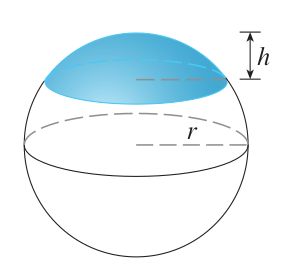
\includegraphics[width=0.3\textwidth]{lista-13-fig1.png}
        \end{figure}
\end{enumerate}
\end{document}
